\subsection{Corporate Restructuring}

\subsubsection{Restructuring Types and Motivations}

\begin{remark} \hlt{Potential Synergies}
\begin{enumerate}[label=\roman*.]
\setlength{\itemsep}{0pt}
\item Cost synergies: lower costs due to economies of scale, elimination of redundant functions
\item Revenue synergies: from economies of scope (cross-selling of products, reduced competitive pressure)
\end{enumerate}
Inefficiencies and negative synergies may result from diseconomies of scale, loss of focus on core competencies.
\end{remark}

\begin{flushleft}
Types of Corporate Transactions
\begin{tabularx}{\textwidth}{p{6em}|X|X}
\hline
\rowcolor{gray!30}
Transaction & Definition & Motivations \\
\hline 
Investment & 
\xxx Increase size and scope of operations
\xxx Increase revenue, revenue growth rate & 
\xxx Realise synergies
\xxx Increase growth 
\xxx Improve capabilities, secure resources
\xxx Acquire undervalued target \\
\hline
Divestment & 
\xxx Decrease size by shedding div with slower growth, lower profitability, higher risk 
&
\xxx Focus operations and business lines
\xxx Valuation
\xxx Liquidity needs
\xxx Regulatory requirements \\
\hline
Restructuring & 
\xxx No change in size
\xxx Improve cost structure, capital structure
\xxx Enhance profitability
\xxx Increase growth
\xxx Reduce risk &
\xxx Improve returns on capital
\xxx Financial challenges (bankruptcy and liquidation) \\
\hline
\end{tabularx}
\end{flushleft}

\begin{remark} \hlt{Top-Down Driver of Corporate Transactions: High Security Prices}\\
Corporate transactions are cyclical, increasing during economic expansions and decreasing during contractions:
\begin{enumerate}[label=\roman*.]
\setlength{\itemsep}{0pt}
\item Greater CEO Confidence: CEO confidence levels increase in economic expansions where security prices are high. CEO are more likely to execute major corporate actions.
\item Lower Cost of Capital: when stock, bond prices are high, resulting in lower interest expense and less dilution to existing shareholders from debt and equity-financed transactions.
\item Overvalued Stock: higher equity valuation beneficial for equity-financed corporate transactions. 
\end{enumerate}
Empirical studies suggest corporate transactions taken during weaker economic times create more value.
\end{remark}

\begin{remark} \hlt{Top-Down Driver of Corporate Transactions: Industry Shocks}\\
Corporate restructuring occurs during industry shocks, which happens during regulatory changes, technological changes, or changes in growth rate of industry. This may be a reactionary motivation.
\end{remark}

\subsubsection{Types of Corporate Restructurings}

\begin{figure}[H]
\centering
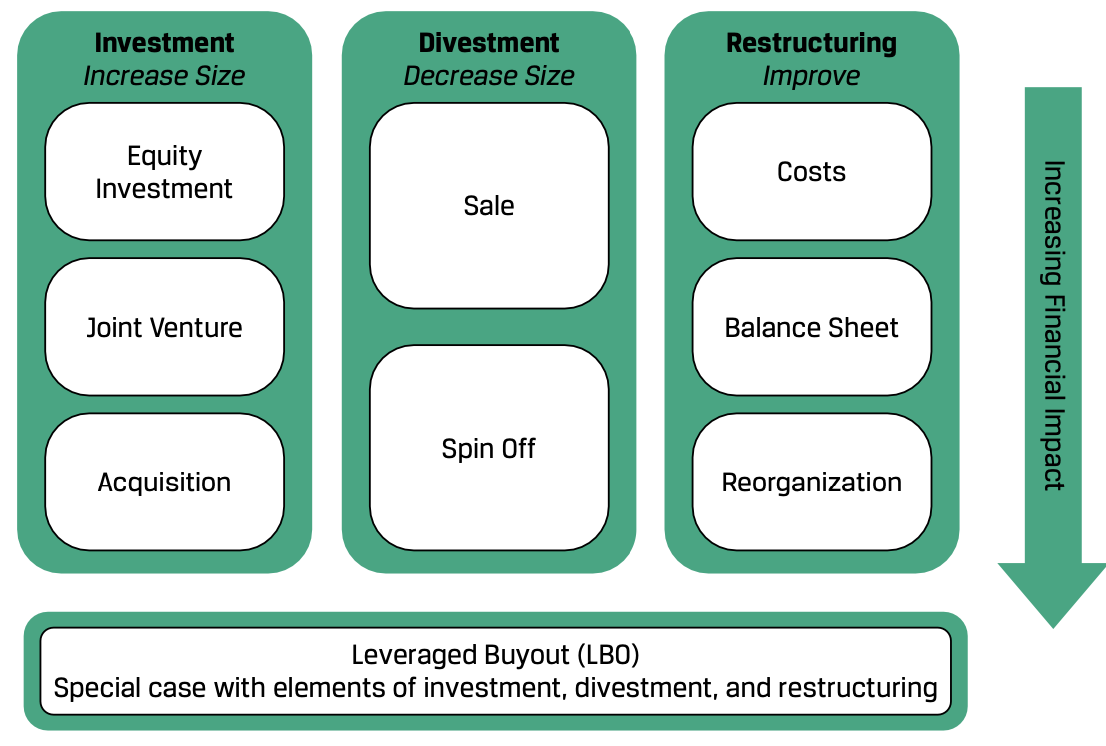
\includegraphics[scale=0.55]{/corpissuer/corprest}
\caption{Types of Corporate Transactions}
\end{figure}

\begin{remark} \hlt{Investment Actions}\\
Acquisitions enable a company to expand quickly, or access inputs at a favourable price.
\begin{enumerate}[label=\roman*.]
\setlength{\itemsep}{0pt}
\item Equity Investment: purchasing material stake in another company with less than 50\% stake. Investor may get board representation in investee, depending on investment size.\\
Equity investment may be made for: establishing strategic partnership between companies, taking initial step towards eventual acquisition, or investment into undervalued company.
\item Joint Venture: two or more companies pool resources, knowledge, or talent, to jointly control a separate, independent company. Usually used by a company seeking to expand into a foreign market, by undertaking with a local company that has existing distribution network and local know-how.
\item Acquisitions: investee becomes subsidiary. Investor company reports consolidated financial statements.
\end{enumerate}
\end{remark}

\begin{remark} \hlt{Divestments}\\
Action of selling off subsidiary business interests. Corporate issuers may have higher valuation if business are separated, due to having conglomerate discount (diseconomies of scale or scope, deficit in focus etc.)
\begin{enumerate}[label=\roman*.]
\setlength{\itemsep}{0pt}
\item Divestiture: sale of division to any company. Seller will no longer have any exposure to the divested business. Sale proceeds may be returned to shareholders, or be put to better use.
\item Spin-Off: creation of new, separate legal entity, distributing equity in newly created spin-off to divesting company shareholders. Spin-off is to improve focus of the management and employees of new company, and allows stock-based compensation schemes to be implemented. No proceeds for divesting company.
\end{enumerate}
Value of divested business is key consideration between a sale and a spin-off. A moderate-to-large-sized business unit sought by several potential acquirers may be able to fetch a high sale price.
\end{remark}

\begin{remark} \hlt{Restructuring}\\
May be forced or opportunistic.\\
Forced restructuring is necessitated by overcapacity, poor management, falling demand, or worsening competitive landscape. Opportunistic restructuring is when the business changes its balance sheet composition, cut costs, or alters business model to improve the return on capital.
\begin{enumerate}[label=\roman*.]
\setlength{\itemsep}{0pt}
\item Cost Restructuring: usually occurs after periods of underperformance. Company pursues improvement in operational efficiency. May be achieved via outsourcing or offshoring.
\begin{enumerate}[label=\arabic*.]
\setlength{\itemsep}{0pt}
\item Outsourcing: contracting out standardised business process to third-party vendors that have lower costs due to their economies of scale. Risk is need to manage multiple contractual obligations.
\item Offshoring: cheaper foreign labour used, while keeping business process in-house.
\end{enumerate}
Outsourcing and offshoring often combined, with a business process outsourced to a foreign company.
\item Balance Sheet Restructuring: changing mix of assets, capital structure.
\begin{enumerate}[label=\arabic*.]
\setlength{\itemsep}{0pt}
\item Sale Leaseback: asset owner sells an asset to lessor for cash, enter lease contract over remaining economic life of asset. Lessee receive cash up front. Lease payment should be higher than depreciation of the asset, reflecting interest charged by lessor. When lessors can secure capital at lower cost, they may offer lessee more attractive financing terms than what lessee could have obtained. Used to secure liquidity on relatively short notice.
\item Dividend Recapitalisation: increasing leverage by increasing debt-financed dividends or by repurchasing shares. Objective is to replace equity in capital structure with cheaper debt, hence lowering WACC. More appropriate for issuers with stable cash flows due to higher risk.
\end{enumerate}
\item Reorganisation: may be mandated by court during insolvency proceeding. Management's reorganisation plan (with terms of exiting bankruptcy proceeding) must be approved by court. Court then oversees measures such as asset sales, refinancing, or conversion of debt to equity. If court does not approve management plan, company may be liquidated.
\end{enumerate}
\end{remark}

\begin{remark} \hlt{Leveraged Buyout (LBO)}\\
Special corporate restructuring involving investment, divestment, and restructuring.\\
PE firm purchases a company using large amount of debt to finance the transaction.\\ 
Unrelated parts are then sold to generate cash to service the debt.\\
Reorganisation of remaining business operations then performed to generate synergies.\\
Eventual exit via sale or public listing.
\end{remark}

\subsubsection{Evaluation of Corporate Restructuring}

\begin{figure}[H]
\centering
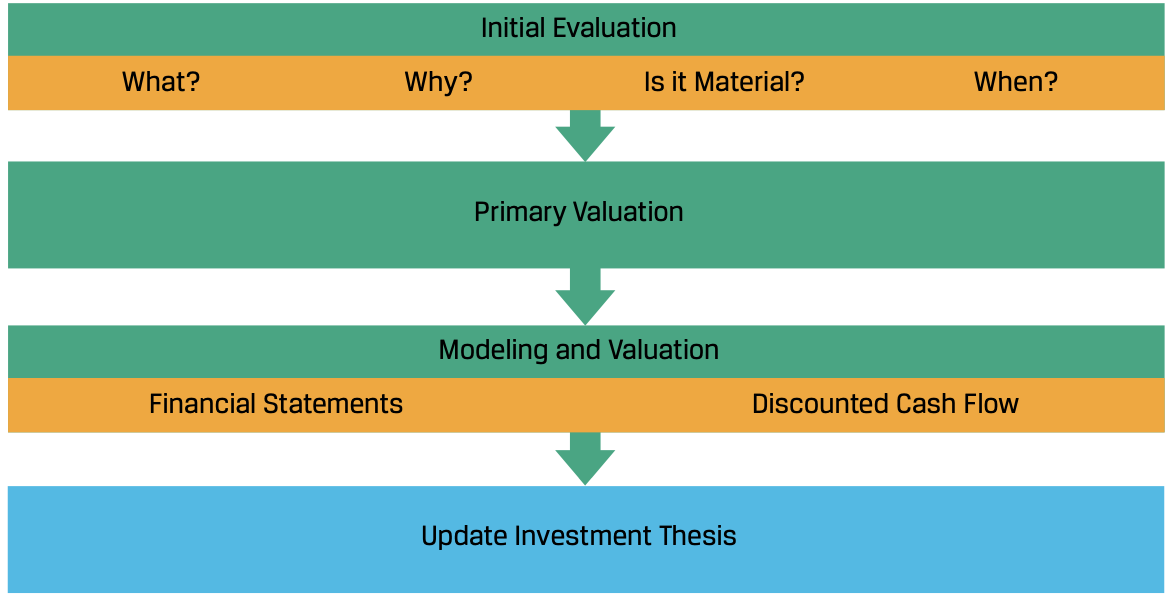
\includegraphics[scale=0.55]{/corpissuer/corpresteval}
\caption{Steps for Evaluating a Corporate Structural Change}
\end{figure}

\begin{remark} \hlt{Initial Evaluation}\\
To determine motivations behind corporate restructuring, data may be retrieved from corporate press releases, securities filings, analyst conference calls.\\
Materiality of corporate restructuring may be evaluated in terms of size (value of transaction as proportion of EV, estimated savings as a percentage of sales) and fit within existing company strategy.\\
Change in stock price when restructuring is announced is an indicator of value that the market expects to be created or destroyed. The change incorporates market estimate of probability of transaction completion, as well as time required for restructuring to finish. 
\end{remark}

\begin{method} \hlt{Primary Valuation: DCF Analysis}\\
Estimate target's future FCF using estimates of earnings, capital expenditures, working capital investments etc. These FCF are discounted to generate an estimate of value. More details in Equity section.
\end{method}

\begin{method} \hlt{Primary Valuation: Comparable Company Analysis}\\
Relative valuation metrics of comparable firms used to estimate value, and takeover premium added.
\begin{enumerate}[label=\arabic*.]
\setlength{\itemsep}{0pt}
\item Identify comparable firms from same industry, with similar size, growth rate, operating margin, and ROIC.
\item Calculate relative value measures based on current market prices of companies in the sample. May use relative value measures based on EV (EV to EBITDA, EV to FCF), equity multiples (PE ratio), sector-specific measures (EV to subscribers for tech, EV to reserves for oil and gas).
\item Apply mean or median multiple to develop estimated target value.
\end{enumerate}
As estimated value of target does not include control or takeover premium, this is used in spin-off valuation.
\end{method}

\begin{method} \hlt{Primary Valuation: Comparable Transaction Analysis}\\
Similar to comparable company analysis, but uses actual transaction prices rather than market prices of stock. Comparable are actual takeover targets. Transaction prices already include takeover premium.
\end{method}

\begin{flushleft}
Comparable Analysis Comparison
\begin{tabularx}{\textwidth}{p{6em}|p{17em}|X}
\hline
\rowcolor{gray!30}
& Comparable Company Analysis & Comparable Transaction Analysis \\
\hline 
Advantages &
\xxx Data for comparable easy to access
\xxx Sound assumption that similar assets have similar values
\xxx Estimates of value derived directly from market, rather than assumptions and estimates about future &
\xxx No need to estimate separate takeover premium
\xxx Estimates of value derived directly from recent actual deals, rather than assumptions and estimates about the future \\
\hline
Disadvantages & 
\xxx Implicit assumption that market valuation of comparables is fair
\xxx Comparables provide estimate of fair stock price, not fair takeover
\xxx Takeover premium calc. separately
\xxx Target may be unique, no true peers &
\xxx Implicit assumption that M\&A market valued past transactions fairly.
\xxx There may not be enough comparable transactions to develop reliable estimate of target value.
\xxx Historical transactions might have occured under different conditions; not representative. \\
\hline
\end{tabularx}
\end{flushleft}

\begin{method} \hlt{Primary Valuation: Premium Paid Analysis}\\
Acquiring firm pays premium over current market price as incentive for target to accept offer.
\begin{equation}
\text{Takover Premium} = \frac{(DP - SP)}{SP} \nonumber
\end{equation}
where $DP$ is deal price per share of target, $SP$ is unaffected stock price of target.\\
Some effect of pre-announcement rumours may be incorporate in trading price; to use week-old market price or volume-weighted trading price over prior week as $SP$ to mitigate the issue.
\end{method}
